%===============================================================================
% Zweck:    KTR-Seminar-Vorlage
% Erstellt: 16.10.2007
% Updated:  27.06.2016
% Autor:    U.K. / M.G.
%===============================================================================
\RequirePackage[hyphens]{url}
\documentclass[journal, onecolumn, a4paper, 12pt]{IEEEtran}
%===============================================================================
% zentrale Layout-Angaben und Befehle
%===============================================================================
\newcommand\meta{./meta}
\newcommand\images{./meta/images}

%===============================================================================
% Zweck: KTR-Seminar-Vorlage in Anlehung an G. Wirtz, Lehrstuhl Praktische Informatik
%===============================================================================
%===============================================================================
% zentrale Layout-Angaben und Befehle
%===============================================================================

% Language Selection for Babel
\usepackage[english,ngerman]{babel}

\makeatletter
\newcommand{\newlanguagecommand}[1]{%
  \newcommand#1{%
    \@ifundefined{\string#1\languagename}
      {``No def of \texttt{\string#1} for \languagename''}
      {\@nameuse{\string#1\languagename}}%
  }%
}
\newcommand{\addtolanguagecommand}[3]{%
  \@namedef{\string#1#2}{#3}}
\makeatother

\newlanguagecommand{\algo}
\addtolanguagecommand{\algo}{english}{Algorithm}
\addtolanguagecommand{\algo}{ngerman}{Algorithmus}
\newlanguagecommand{\loa}
\addtolanguagecommand{\loa}{english}{List of Algorithms}
\addtolanguagecommand{\loa}{ngerman}{Algorithmen}
\newlanguagecommand{\abbr}
\addtolanguagecommand{\abbr}{english}{List of Abbreviations}
\addtolanguagecommand{\abbr}{ngerman}{Abk\"urzungsverzeichnis}
\newlanguagecommand{\uni}
\addtolanguagecommand{\uni}{english}{University of Bamberg}
\addtolanguagecommand{\uni}{ngerman}{Otto-Friedrich-Universit\"at Bamberg}
\newlanguagecommand{\chair}
\addtolanguagecommand{\chair}{english}{Professorship for Computer Science}
\addtolanguagecommand{\chair}{ngerman}{Professur f\"ur Informatik}
\newlanguagecommand{\chairsub}
\addtolanguagecommand{\chairsub}{english}{Communication Services, Telecommunication\\[.5em]%
Systems and Computer Networks}
\addtolanguagecommand{\chairsub}{ngerman}{insbesondere Kommunikationsdienste,\\[.5em]%
Telekommunikationsdienste und Rechnernetze}
\newlanguagecommand{\seminar}
\addtolanguagecommand{\seminar}{english}{Seminar on}
\addtolanguagecommand{\seminar}{ngerman}{Ausarbeitung des KTR-Seminars}
\newlanguagecommand{\topic}
\addtolanguagecommand{\topic}{english}{Topic}
\addtolanguagecommand{\topic}{ngerman}{Thema}
\newlanguagecommand{\submitter}
\addtolanguagecommand{\submitter}{english}{Submitted by}
\addtolanguagecommand{\submitter}{ngerman}{Vorgelegt von}
\newlanguagecommand{\lsupervisor}
\addtolanguagecommand{\lsupervisor}{english}{Supervisor}
\addtolanguagecommand{\lsupervisor}{ngerman}{Betreuer}

% What You should change:
% Here goes your name
\author{Author}
% and the title of your seminar
\newcommand{\subtitle}{Your Topic on the Seminar}
% the date of the submission
\date{\today}

% What is already done

\newlanguagecommand{\semester}
\addtolanguagecommand{\semester}{english}{Summer Term 2017}
\addtolanguagecommand{\semester}{ngerman}{Sommersemester 2017}

\newlanguagecommand{\ltitle}
\addtolanguagecommand{\ltitle}{english}{Fog Computing for Internet-of-Things Applications}
\addtolanguagecommand{\ltitle}{ngerman}{Fog Computing for Internet-of-Things Applications}

\title{\ltitle}
\newcommand{\supervisor}{Prof. Dr. Udo Krieger}

\gittrue
\seminartrue


\usepackage[utf8]{inputenc}
\usepackage{fancyhdr}
\usepackage[T1]{fontenc}
\ifgit
  \usepackage[mark]{gitinfo2}
\fi
\usepackage{ae}
\usepackage{color}
\usepackage{amsmath}
\usepackage{amsfonts}

%%   Fuer anspruchsvolle Tabellen   %%
\usepackage{longtable, colortbl}
\usepackage{multicol, multirow}

\usepackage[pdftitle={\@title},pdfauthor={\@author},pdftex,bookmarksopen,bookmarksnumbered]{hyperref}
\usepackage[pdftex]{graphicx}
\usepackage{float}
\usepackage{tikz}
\usepackage{pgfplots}
\usetikzlibrary{arrows,shapes,fit,positioning,decorations,backgrounds,shadows}

\pdfcompresslevel=9

% Code-Hervorhebung
% Quellcode
\usepackage{verbatim}            % Quellcode einbinden (\verbatiminput) standardpaket
\usepackage{moreverb}
% PseudoCode
\usepackage{algorithm}
\usepackage{algpseudocode}
%\usepackage{algorithmicx}

\floatname{algorithm}{\algo}
\algrenewcommand{\algorithmiccomment}[1]{\hskip1em\textcolor{gray!60}{$\rhd$ #1}}
\renewcommand{\listalgorithmname}{\loa}
\def\algorithmautorefname{\algo}


%%   intoc zur Aufnhame des Abkuerzungs- und Symbolverzeichnisses ins Inhaltsverzeichnis
\usepackage[intoc]{nomencl}
\setlength{\nomlabelwidth}{.20\hsize}
\renewcommand{\nomlabel}[1]{#1 \dotfill}
\setlength{\nomitemsep}{-\parsep}
\makenomenclature

\renewcommand{\nomname}{\abbr}

%%   Hervorhebung der Abkuerzungsbuchstaben   %%
\usepackage[normalem]{ulem}
\newcommand{\m}[1]{\uline{#1}}

% ausf\"{u}hrlichere Fehlermeldungen
\errorcontextlines=999
%
% Page-Layout: A4 aus Header
% Alternative
\setlength\headheight{14pt}
\setlength\topmargin{-15,4mm}
\setlength\oddsidemargin{-0,4mm}
\setlength\evensidemargin{-0,4mm}
\setlength\textwidth{160mm}
\setlength\textheight{252mm}
%
%% Absatzeinstellungen
\setlength\parindent{0mm}
\setlength\parskip{2ex}



\makeatletter
\renewcommand{\maketitle} {
  \begin{titlepage}
  \centering
    \begin{minipage}[t]{16cm}
      \hfill
      \begin{minipage}{12cm}
            \centering
        \uni
        \\[12pt]%
        {\Large \chair\\[.5em]%
        \large \chairsub}%
      \end{minipage}
      \hfill
      \begin{minipage}{3cm}
        
\includegraphics[height=28mm]{config/images/logo} %height=26mm
      \end{minipage}
    \end{minipage}\\[70pt]%[50pt]
    {\Large\bf \seminar}
    \\[36pt]
    {\LARGE \@title}\\[80pt]
    {\Large\bf \topic:}\\[36pt]
    {\LARGE\bf \subtitle}\\
    \vfill
    \begin{minipage}{\textwidth}
      \center
      \submitter:\\
      {\Large \@author \\[18pt]}
      \lsupervisor: \supervisor \\[12pt]
      Bamberg, \@date\\
      \semester
    \end{minipage}
  \end{titlepage}
}
\makeatother
%

% Einbindung eines Bildes mit angegebener Breite
% #1 = label f\"{u}r \ref-Verweise
% #2 = Name des Bildes ohne Endung relativ zu Bilder-Verzeichnis
% #3 = Beschriftung
% #4 = Breite des Bildes im Dokument in cm
\newcommand{\bildw}[4]{%
  \begin{figure}[htb]%
    \centering
    \includegraphics[width=#4cm]{Bilder/#2}%
    \vskip -0.3cm%
    \caption{#3}%
    \vskip -0,2cm%
    \label{#1}%
  \end{figure}%
}
%
% Einbindung eines Bildes mit Seitenbreite
% #1 = label f\"{u}r \ref-Verweise
% #2 = Name des Bildes ohne Endung relativ zu Bilder-Verzeichnis
% #3 = Beschriftung
\newcommand{\bild}[3]{%
  \begin{figure}[htb]%
    \centering%
    \includegraphics[width=\textwidth]{Bilder/#2}%
    \vskip -0.3cm%
    \caption{#3}%
    \vskip -0,2cm%
    \label{#1}%
  \end{figure}%
}
%
\numberwithin{equation}{section}
%
%===============================================================================
% zentrale Layout-Angaben und Befehle
%===============================================================================
%
%#1 Breite
%#2 Datei (liegt im image Verzeichnis)
%#3 Beschriftung
%#4 Label fuer Referenzierung
\newcommand{\image}[4]{%
\begin{figure}[H]%
\centering%
\includegraphics[width=#1]{image/#2}%
\caption{#3}%
\label{#4}%
\end{figure}%
}

%#1 Datei (liegt im graphic Verzeichnis)
%#2 Beschriftung
%#3 Label fuer Referenzierung
%#4 Skalierungsfaktor
\newcommand{\scaletikzimage}[4]{%
\begin{figure}[H]%
\centering%
\scalebox{#4}{%
\input{graphic/#1.tikz}}%
\caption{#2}%
\label{#3}%
\end{figure}
}

%#1 algorithm name
%#2 algorithm label
%#3 file name in code-folder
\newcommand{\pseudo}[3]{%
\small%
\begin{algorithm}[H]%
\caption{#1}%
\label{#2}%
\input{code/#3.tex}%
\end{algorithm}%
\normalsize%
}


%===============================================================================
% LATEX-Dokument
%===============================================================================
\hyphenation{op-tical net-works semi-conduc-tor}
\begin{document}
  %===============================================================================
  % Zum Kompilieren pdflatex und bibtex ausführen.
  % Konfiguration in texmaker: Options -> Configure Texmaker -> Quick Build -> Select Latexmk + ViewPDF
  % Entsprechende Informationen in den config/metainfo verändern
  % Zur Auswahl der Sprache im folgenden Befehl
  % ngerman für deutsch eintragen, english für Englisch.
  %===============================================================================
\selectlanguage{english}

\maketitle

\pagenumbering{Roman}
\setcounter{page}{2}
%
\tableofcontents
% Einstellungen f\"{u}r Literaturverzeichnis
\newpage
\addcontentsline{toc}{section}{\listfigurename}
\listoffigures
\newpage
\addcontentsline{toc}{section}{\listtablename}
\listoftables
\newpage
\printnomenclature
%===============================================================================
% LATEX-Dokument: Kapitel laden
%===============================================================================
%
\newpage
\pagenumbering{arabic}
\setcounter{page}{1}
%
% to use git tagging
%
%\ifgit
%      \section{VERSION}
    \subsection{git}
    \#: \gitAbbrevHash\\
    @: \gitAuthorIsoDate\\
    \gitReferences
    \subsection{gitinfo2 -- setup}
    \url{https://www.ctan.org/tex-archive/macros/latex/contrib/gitinfo2}
    \subsubsection{git hooks}
    To fill watermark at buttom, deploy gitinfo2-hook.txt to githooks: (copy and make executable)
    \begin{itemize}
        \item .git/hooks/post-checkout
        \item .git/hooks/post-commit
        \item .git/hooks/post-merge
    \end{itemize}
    \subsubsection{remove watermark}
    To disable watermark, remove option \texttt{[mark]} from \textbackslash usepackage[mark]\{gitinfo2\} in \textit{config/commands.tex} at line 45.

%\fi
%
% hier einzelne Kapitel mit \input{Kapitel-File} einf\"{u}gen
%
%===============================================================================
% Zweck:    KTR-Seminar-Vorlage
% Erstellt: 16.10.2007
% Autor:    U.K.
%===============================================================================
% Abschnitt 1:
%===============================================================================
\section{Architektur optischer Netze der n\"achsten Generation} 
%===============================================================================
%
Original title: Bio-inspired Information and Communications Technology and Swarm Intelligence in Next Generation Networks
\\

%===============================================================================
\subsection{Optische Dienste der n\"achsten Generation} 
%===============================================================================
%
Original title: Bio-inspired Information and Communications Technology and Swarm Intelligence in Next Generation Networks
\\
\nomenclature{NGN}{Next Generation Network}%


Summarize the contents and explain the technical items.

Citation: \cite{Ferstl.2006}
\section{Architecture Overview}

In this chapter, we will review the architectures of Multi-access Edge Computing and the enabling key technologies like Network Functions Virtualization.

\subsection{Introduction to Multi-access Edge Computing}

\begin{figure}[H]
	\centering
	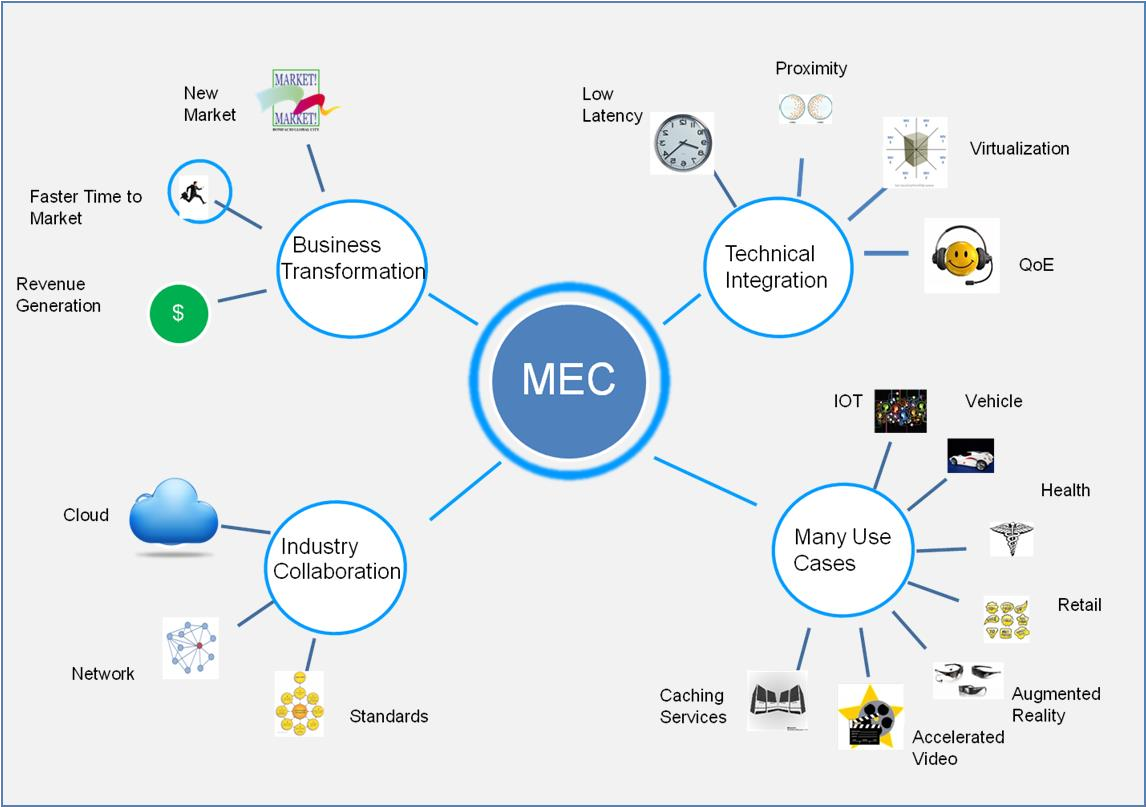
\includegraphics[width=0.9\textwidth]{mec_market_drivers}
	\label{fig:3}
    \caption{MEC Market Drivers \protect\cite{mec5g}}
\end{figure}

Edge Computing refers to carrying out complete or part of the computation at the edge device instead of moving the data to the data center or cloud. There are obvious advantages to this methodology. The key advantage being effective bandwidth utilization due to proximity of data sources to the computation center. It also allows for new kind of services that reside on the edge giving rise to applications in the area of health care, automotive, industrial automation and mobile gaming along with the new and upgraded telecommunication services. 

While MEC emerged as a key enabler for 5G technology, it has broad applications in 4G deployments as well and when paired with other technologies like Cloud RAN, NFV, IOT, a whole new horizon of new service possibilities emerges. 

\subsection{MEC Architecture}

ETSI establishes a reference framework and architecture to realize MEC as shown below:

\begin{figure}[h!]
    \centering
    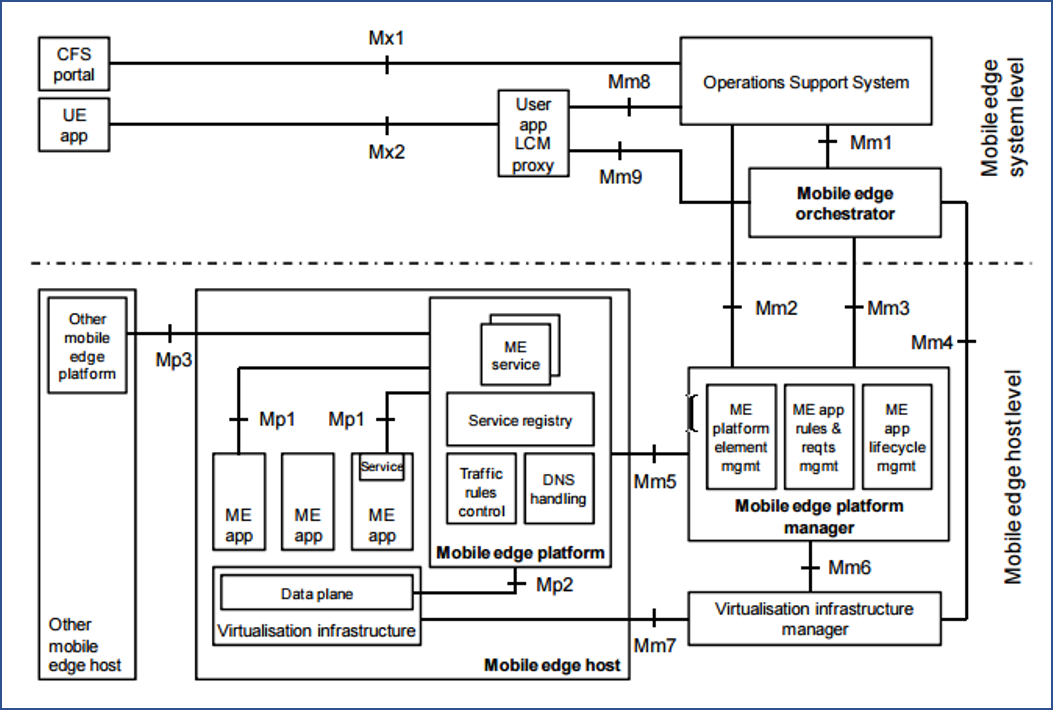
\includegraphics[width=0.9\textwidth]{mec_ref_architecture}
    \label{fig:figure4}
    \caption{ETSI MEC Reference Architecture}
\end{figure}

The architecture comprises the following 4 components:
\begin{enumerate}
    \item \textit{The MEC host} – provides the necessary infrastructure including virtualized resources.
    \item \textit{The MEC Platform} – Provides functionality and interfaces to run applications on top of the MEC host.
    \item \textit{MEC Management} – Handles host and system level management. It can be done at two levels – the host level involving the platform manager and the infrastructure manager and the system level using the MEC Edge orchestrator.
    \item \textit{MEC Applications} – Are services provided through the MEC architecture some of which can also be provided by the MEC platform manager.
\end{enumerate}

\subsection{NFV Architecture}

The goal of NFV  is to be able to run network services traditionally hosted in specialized hardware in virtualized resources like virtual machines and containers. This gives the necessary flexibility for realizing use-cases discussed above.  The following figure shows the reference architecture of a typical NFV deployment. The essential framework is outlined by etsi at \cite{etsi02}.

\begin{figure}[h!]
	\centering
	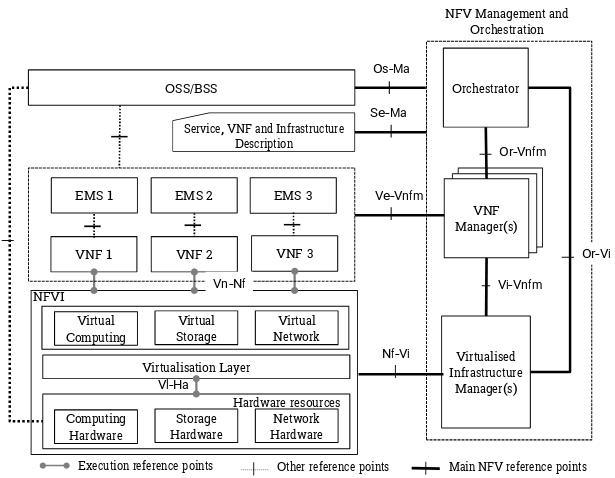
\includegraphics[width=0.9\textwidth]{nfv_ref_architecture}
	\label{fig:figure5}
    \caption{ETSI NFV Reference Architecture \cite{etsi02}}
\end{figure}

The NFV Architecture Framework in~\ref{fig:figure5} is a reference for designing an NFV solution and proposes the following components:

\begin{enumerate}
    \item \textit{Virtual Network Function}
        The functionality that traditionally runs on dedicated hardware and is intended to be virtualized. The functions could be the basic Enterprise functions like Firewall, DNS etc or specialized telecommunication functions like packet processing, mobility management etc,. The VNF can run on a single entity like a virtual machine or a container or on a cluster of virtual machines or containers. The functions that use containers as compute resources are sometimes referred to as Containerized Network Functions (CNF). 
    \item \textit{Element Management}
        The Element Management unit can be used to manage single of multipl VNF units for combined functionality. 
    \item \textit{NFV Infrastructure}
        NFVI refers to the virtualization infrastructure resources providing the compute, network and storage requirements of the VNFs. The infrastructure could comprise of Virtual Machines or Containers, Block and Object Storage units, Network artifacts and the hardware resources that hosts these resources.   
    \item \textit{Virtualized Infrastructure Manager}
        The VIM provides the management functions for the virtualized infrastructure. The functions include inventory management, resource allocation, monitoring, capacity planning, fault management, resource optimization and policy management.
    \item \textit{NFV Orchestrator}
        The Orchestrator is responsible for translating the requirements of a VNF into corresponding resources on the Virtualized Infrastructure. A standard format of description can be used for describing the requirements that can be answered by different VIM solutions.
    \item \textit{VNF Manager}
        The VNF Manager manages the lifecycle of the VNF including instantiation, update, query, scaling, termination and service availability
    \item \textit{Service, VNF and Infrastructure Description}
        This describes a model to describe the entities in the NFV architecture including the Service, VNF and the Infrastructure. The model should be standard and universal so that the same description can be used to abstractly realize multiple types of infrastructure solutions. 
    \item \textit{Operations and Business Support Systems - OSS/BSS}
        The Orchestration and Management blocks of the NFV reference architecture are expected to expose standard APIs for applications. The set of applications that monitor and collect various measurement data from the NFV system can also provide for operational and business functions like service provisioning, billing, auditing etc,. that are essential functions for an operator in order to monetize the solution offered through NFV.
\end{enumerate}

\subsection{Combined Architecture for NFV an MEC}

\begin{figure}[ht!]
    \centering
    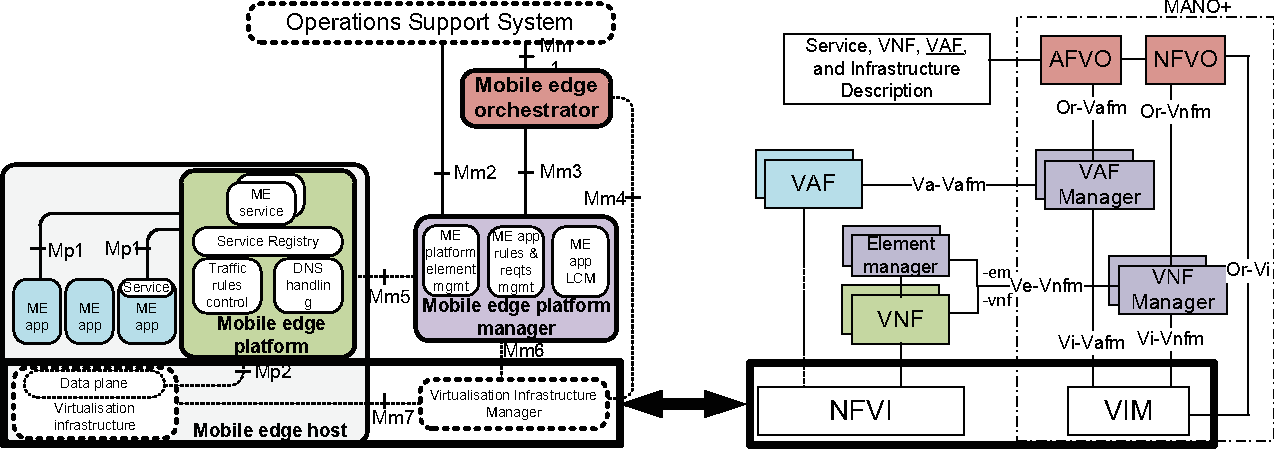
\includegraphics[width=0.9\textwidth]{images/combined_architecture}
    \label{fig:figure6}
    \caption{A Combined architecture for NFV and MEC \protect\cite{taleb17}}
\end{figure}

The NFV Infrastructure provides the necessary foundation for realizing all the pillars including MEC and NFV\@. The infrastructure mainly provides functions to automatically deploy and manage virtualized resources. Several requirements for NFV and MEC overlap and due to the similarities, a combined architecture for NFV and MEC was proposed in \cite{taleb17}. The idea is to use a common Infrastructure platform to run Virtual Application Functions (VAFs) and Virtual Network Functions (VNFs). The corresponding orchestration modules are named as AFVO and NFVO\@. This common platform allows for reduced design issues and massive reuse of components thereby saving in CapeX and OpeX costs. A paper in [2] represents a combined architecture as in the above diagram.


Here is a table comaparing the terminologies used between NFV and MEC

\begin{longtable}{||p{0.2\textwidth}|p{0.2\textwidth}|p{0.2\textwidth}||}
\hline\hline
\textbf{Component}&\textbf{NFV}&\textbf{MEC} \\
\hline
Managed Entity&VNF&VAF \\
\hline
Orchestrator&NFVO&AFVO \\
\hline
Platform Manager&VNF Manager&VAF Manager \\
\hline
Infrastructure&NFV Infrastructure&Mobile Edge Host \\
\hline\hline
\label{tab:tab2}
\caption{Comparing terms for NFV and MEC in a common reference architecture \cite{taleb17}}
\end{longtable}

\section{Requirements for NFV}
\begin{flushleft}

The variety of use-cases that NFV claims to support and the nature of the functions that run as VNFs demands for certain requirements to be met. ETSI has drafted several requirements and these can be classified under 4 categories. These requirements are laid out taking into consideration both the functioning of the NFV system as well as the Service Level Agreements (guarantees) that such a system is obligated to provide its consumers.
\end{flushleft}

\newpage
\subsection{Hardware requirements}
\begin{flushleft}
ETSI specifies considerations \cite{etsi04}  while choosing or adapting the telecommunications for NFV workloads. The environments include Central Office, Access Node, Transport Node and Data Center. Since majority of the NFV functions are expected to be implemented in the Data Center, the hardware requirements focuses on the requirements for the Data Center. One of the key goals is the ability to run Network Functions on COTS (Commercial Off The Shelf) hardware without vendor-locking and licensing issues. The second key consideration is interoperability so that workloads can be moved to different hardware automatically without performance or functionality impact. This is also necessary to achieve high level of resiliency. 
\end{flushleft}

\subsection{Virtualization requirements}
	
\begin{flushleft}
The network functions are expected to be run in one or more virtual resources. There are two competing technologies that help process the computation workloads for the VNFs – Virtualization and Containers. The nature of computation and traffic that is handled by NFV demands very high and deterministic performance. Its not sufficient to provide high speed but also real-time capability with reduced jitter. Jitter is defined as the deviation in the promised latency (the response time for the data processing unit).  
	
Operating the NFV system requires several actions to be performed on the virtualized resources (Virtual Machines or Containers). Hence these requirements dictate the metrics expected on various operations like below:
\end{flushleft}

\begin{enumerate}
    \item Inter-VM communication
    \item VM to host 
    \item VM boot time
    \item VM migration across hosts
    \item Security
\end{enumerate}


Since the virtualization is responsible for processing the NFV workloads, it is important to understand the classification of Workloads as outlined by ETSI in Figure [] below.

The introduction of Software Defined Networking technology in the mix, the network functions are separated into Control Plane and Data Plane. While the control plane is responsible for computing the destination, routing, tunneling and other control functions of the data transfer process, the data plane focuses on the forwarding of the packets as instructed by the control plane. The interface between the control and data plane are well defined either through standardized protocols or APIs. The details of the SDN solution and its role in NFV is discussed in a later section. 

	
\subsection{Resiliency requirements}

Telecommunication functions demand high resiliency against various threats including disaster, failures, loss of communication, errors and overloading of resources. The resiliency requirements define measures that could be taken at each level including hardware failures, virtualization, IaaS and the VNF\@. The management and orchestration functions provide external modules that support such high-resiliency requirements. IaaS solutions have in-built solutions and external or third party supported integrations that provide high availability and resiliency. Specific components to realize this requirement for various IaaS solutions are discussed in later sections.

	
\subsection{Management and Orchestration requirements}

Apart from resiliency of the Virtual Network Functions, the Orchestration module is also responsible for many other functions for effective life cycle management of the VNFs. Some of these include provisioning, monitoring, fault detection and recovery, policy management and service chaining/clustering as required by the specific services.

\section{Enabling Technologies}

A range of technologies developed over several years have enabled the evolution of NFV and Edge Computing. This seections briefly describes and compares the technologies that led to the development of MEC and its parallel technology NFV.

These technologies can be grouped into 4 different planes based on their functionalities.

\begin{enumerate}
    \item Data Plane
	\begin{itemize}
	    \item Follows the forwarding logic and responsible for physically moving the packets in the network.
        \end{itemize}
    \item Control Plane
	\begin{itemize}
	    \item Computes the forwarding logic as required by the other planes and programs them to the Data plane and monitors the data plane.
        \end{itemize}
    \item Management Plane
	\begin{itemize}
	    \item Responsible for orchestration and management of resources as required by the services.
	\end{itemize}
    \item Application Plane
	\begin{itemize}
	    \item Makes use of the services through Service Abstraction and APIs from Management to deliver end-user applications.
	\end{itemize}
\end{enumerate}

These planes are depicted in the figure below in Figure 6.

\begin{figure}
	\centering
        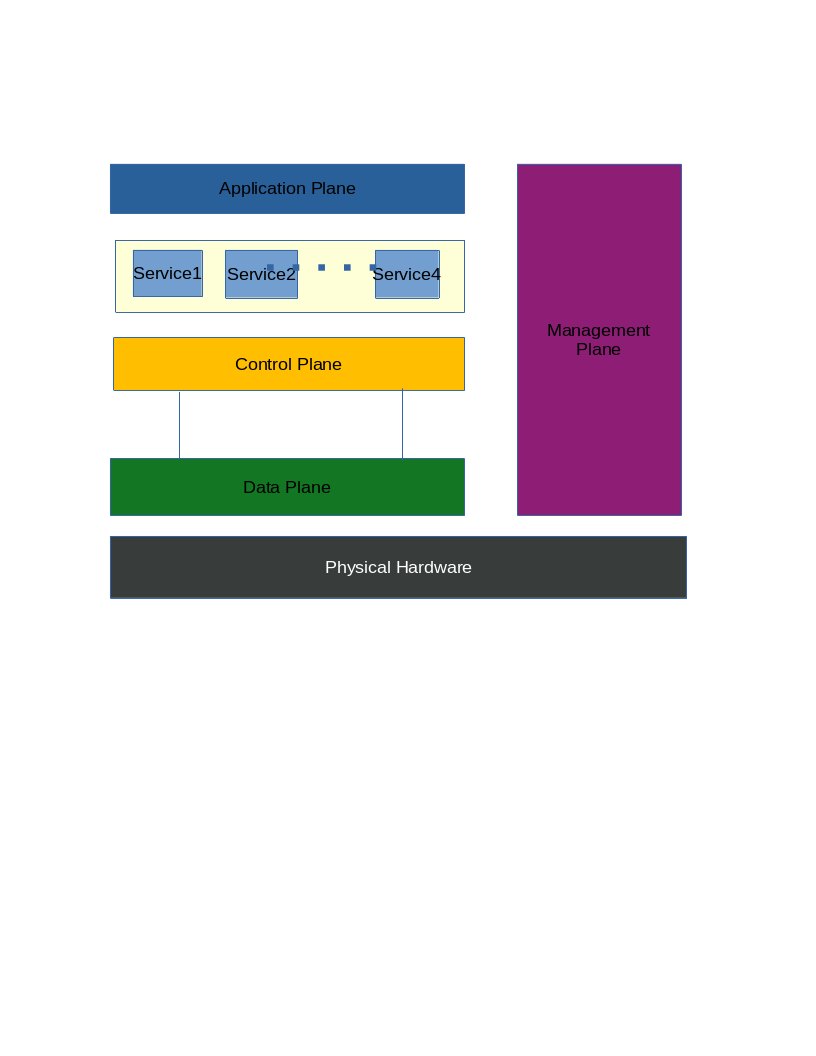
\includegraphics[width=0.7\textwidth]{planes_of_computing}
	\label{fig:figure6}
	\caption{Planes of NFV and MEC Architectures}
\end{figure}

The architecture also evolves into multiple business models as envisaged by the NIST Cloud Computing group

\begin{enumerate}
    \item Infrastructure As A Service
    \item Platform as a Service
    \item Software As A Service
\end{enumerate}

\subsection{NFV Infrastructure}

\begin{flushleft}	
The NFV Infrastructure provides the necessary foundation for realizing all the pillars including MEC and NFV\@. The infrastructure mainly provides functions to automatically deploy and manage virtualized resources. Several requirements for NFV and MEC overlap and due to the similarities, a combined architecture for NFV and MEC was proposed in [2]. The idea is to use a common Infrastructure platform to run Virtual Application Functions (VAFs) and Virtual Network Functions (VNFs). The corresponding orchestration modules named as AFVO and NFVO\@. This common platform allows for reduced design issues and massive reuse of components thereby saving in CapeX and OpeX costs.
\end{flushleft}

\newpage
\subsection{NFV Workloads}

\begin{figure}[h!]
    \centering
    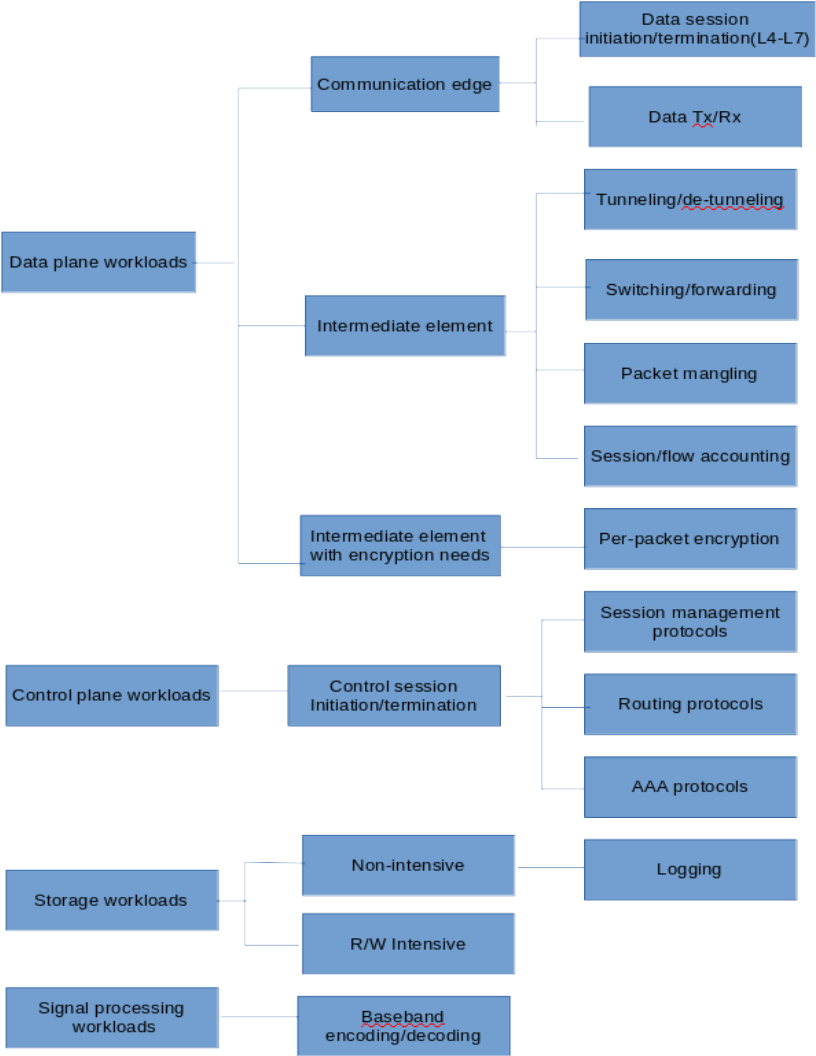
\includegraphics[width=0.9\textwidth]{workload_classification}
    \label{fig:8}
    \caption{Classification of various workloads running on NFVI \protect\cite{etsi01}}
\end{figure}

\subsection{Virtualization}

A basic layered architecture of the Virtual Machines running application workloads is as below in [Fig. 10] based on the explanation from [3]

\begin{figure}[h!]
    \centering
    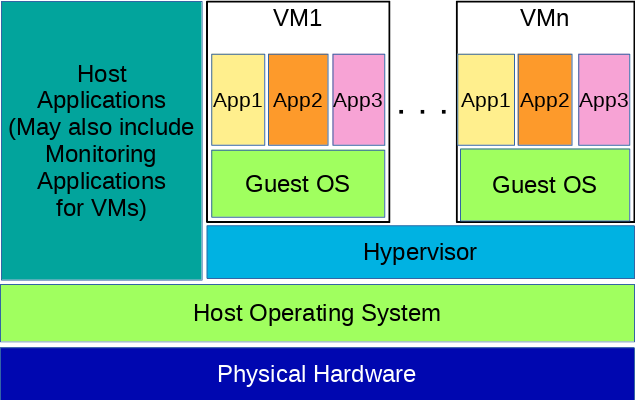
\includegraphics[width=0.5\textwidth]{vm_layers}
    \label{fig:figure9}
    \caption{Components of Virtualization}
\end{figure}

In traditional virtualization, also refered to as hardware virtualization, a hypervisor (eg: KVM) emulates the hardware into a guest and isolates it from other KVM instances. An Operating System can be installed and the KVM instance can then be used as an independent system for any application. The interaction between the application running on the Guest Operating system and the host operating system kernel is through the intermediate interface called the Hypercall. The hypervisor needs a virtual switch which it can connect to using tap interfaces to communicate with other Virtual Machines (KVM instances). Libraries such as Libvirt provide interfaces to interact with the KVM instances with ease.

\subsection{Containerization}

\begin{figure}[h!]
    \centering
    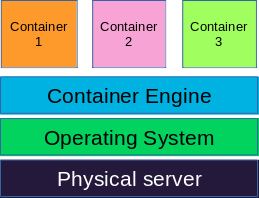
\includegraphics[width=0.5\textwidth]{container_layers}
    \label{fig:10}
    \caption{Components of Containerization \protect\cite{docker}}
\end{figure}

\begin{flushleft}
A Container is a software unit that packages an application along with all its dependencies including libraries, environment and tools necessary to run the application on any computing environment thereby allowing for easy migration from one computing environment to another. Docker provides an eco-system to create images, store them in a repository, run the application and monitor the application on a computing environment. Refer to documentation in [3]
The layered architecture of a container-based system is as in [Fig.11] below based on the explanation from [3]
\end{flushleft}



\section{Evaluation of Virtualization vs Containerization}

\subsection{Qualitative Comparison}
	
\begin{flushleft}
Two competing technologies provide virtual resources to run NFV workloads – Virtual Machines and Containers. [1] (TABLE 1) provides a qualitative comparison of these technologies. Below table [Table 1] is an expansion of the same.

\begin{longtable}[t!]{|p{4cm}|p{4cm}|p{4cm}|}
	
\hline\hline
\textbf{Feature} & \textbf{Virtualization} & \textbf{Containerization} \\
\hline\hline
\hline
Compute Virtualization & Hardware Abstraction & Application Binary Interface \\
\hline
Interaction with the System & Hypervisor-based & System Calls \\
\hline
Base Workload & Complete Guest OS & Processes and Dependencies \\
\hline
Provisioning & Slow and Complex & Fast and Scalable \\
\hline
Resource Consumption & High & Low \\
\hline
Isolation & Full Isolation & Process-Level Isolation \\
\hline
Management & Openstack, AWS, Azure, GCE & Kubernetes, Docker Swarm, Mesos \\
\hline
Single Independent Abstraction & VM Instances & Multi-container PODs \\
\hline\hline
\hline
\label{tab:tab3}
\caption{Qualitative comparison of Virtualization and Containerization. (TABLE1 \cite[p.1663]{taleb17}}
\end{longtable}
	
\end{flushleft}

\subsection{Quantitative Comparison}

\begin{flushleft}
The differentiating factors that aids the decision of using either virtual machines or containers for running the workloads for the desired application depends on the key performance parameters. For use-cases including NFV for telecommunication services and Edge computing applications, the following performance factors are considered important:
\end{flushleft}

\begin{enumerate}
    \item Latency
    \item Throughput
    \item Isolation
    \item Allocation
\end{enumerate}

A table comparing Virtual Machines and Containers on some of the performance parameters is shown below and we can arrive at a Kiviat diagrams that represents such a table.
The comparison is made on the basis of two measures:
\begin{enumerate}
    \item Memory Sizes
    \item Running Time
\end{enumerate}

\newpage
\begin{longtable}[t!]{|p{0.2\textwidth}|p{0.2\textwidth}|p{0.2\textwidth}|}
\hline\hline
Workload Description&Virtual Machines&Containers\\
\hline\hline
\hline
Kernel Compilation Memory Size (in GB)&4.0&0.42\\
\hline
MySQL Image size(in GB)&1.68&0.37\\
\hline
Memory Intensive YCSB&4.0&4.0\\
\hline
CPU Intensive SpecJBB&4.0&1.7\\
\hline
Disk Intensive Filebench&4.0&2.2\\
\hline
\hline\hline
\label{tab:tab4}
\caption{Operational memory size comparison for VMs and Containers \cite{sharma16}}
\end{longtable}

%\begin{tikzpicture}

%\tkzKiviatDiagram[scale=1.0,label distance=3cm,radial=10,gap=0.5,lattice=10]
%	{Kernel Compilation,MySQL Image,Memory Intensive,CPU Intensive,Disk Intensive}
%\tkzKiviatLine[ultra thick,color=green,mark=ball,mark size=4pt,
%               fill=green!20,opacity=0.5](4.0,1.68,4.0,4.0,4.0)
%\tkzKiviatLine[ultra thick,color=red,mark=ball,mark size=4pt,
%               fill=red!20,opacity=0.5](0.42,0.37,4.0,1.7,2.2)
%\tkzKiviatGrad[prefix=,unity=0.5](0.5)

%\end{tikzpicture}

\begin{figure}[h!]
    \centering
    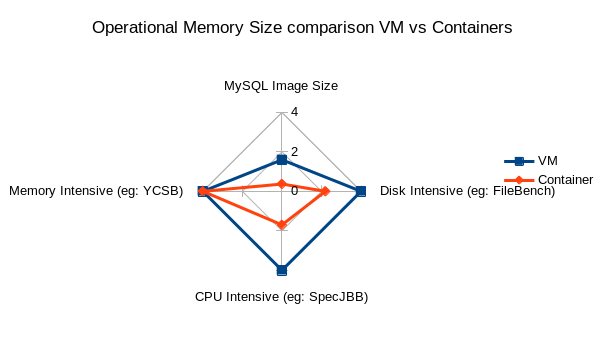
\includegraphics[width=10cm,height=6cm]{memory_size_vm_container}
    \label{fig:12}
    \caption{Comparing VMs and Containers on operational memory size, inspired from \protect\cite{mach17}}
\end{figure}

\newpage
\begin{longtable}[t!]{|p{0.2\textwidth}|p{0.2\textwidth}|p{0.2\textwidth}|}
\hline\hline
\textbf{Workload Description}&\textbf{Virtual Machines}&\textbf{Containers}\\
\hline\hline
\hline
MySQL Image build Time(in sec)&236.2&129\\
\hline
Workload running time (Dist upgrade in sec)&391&470\\
\hline
Workload kernel Install(in sec)&303&292\\
\hline
\hline\hline

\label{tab:tab5}
\caption{Running time comparison for various actions for VMs and Containers \cite{sharma16}}
\end{longtable}

%\begin{tikzpicture}

%\tkzKiviatDiagram[scale=0.01,label distance=3cm,radial=10,gap=1,lattice=10]
%	{MySQL Image Build,Dist Upgrade,Kernel Install}
%\tkzKiviatLine[ultra thick,color=green,mark=ball,mark size=4pt,
%               fill=green!20,opacity=0.5](236,391,303)
%\tkzKiviatLine[ultra thick,color=red,mark=ball,mark size=4pt,
%               fill=red!20,opacity=0.5](129,470,292)
%\tkzKiviatGrad[prefix=,unity=50](50)

%\end{tikzpicture}

\begin{figure}[h!]
    \centering
    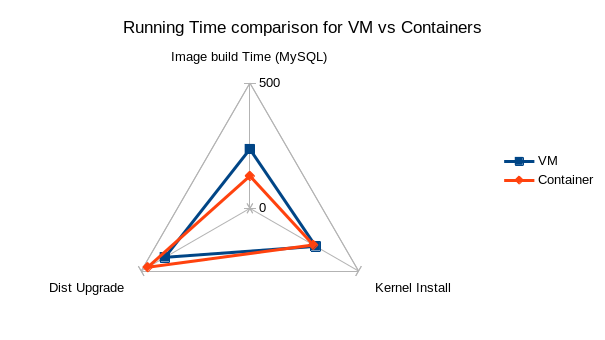
\includegraphics[width=10cm,height=6cm]{time_comparison_vm_container}
    \label{fig:13}
    \caption{Comparison of Running times for activities for VMs vs Containers \protect\cite{mach17}}
\end{figure}

\input{\meta/Content/iaas}
\subsection{OpenStack for IaaS}

OpenStack is an open source Cloud Management solution that utilizes hypervisor-based virtualization technology and provides functions for management of virtualized entities from a central control center. The logical architecture of OpenStack [4] is as below. A typical openstack deployment uses a central controller node with replication and runs all the essential services. Depending on the scale of deployment, these services can either be run on individual nodes or on separate nodes. The services are connected through a common messaging and database architecture and the services are referenced as endpoints. The core computational entities are compute nodes which run agents that communicate with the controller services and host the virtual machines. The controller provides a Graphical User Interface and Command Line Interface to interact with all the services and resources connected to the combined cluster. 

OpenStack is completely written in Python and exposes REST-based APIs which helps integrate with multiple Orchestration or other solutions that need to use OpenStack services and events. OpenStack also integrates with several open source and proprietary underlay technologies for compute, storage and networking through mechanism drivers that are open source components. This is essential for interoperability with existing and new technologies used in enterprise production environments.

\begin{figure}
    \centering
    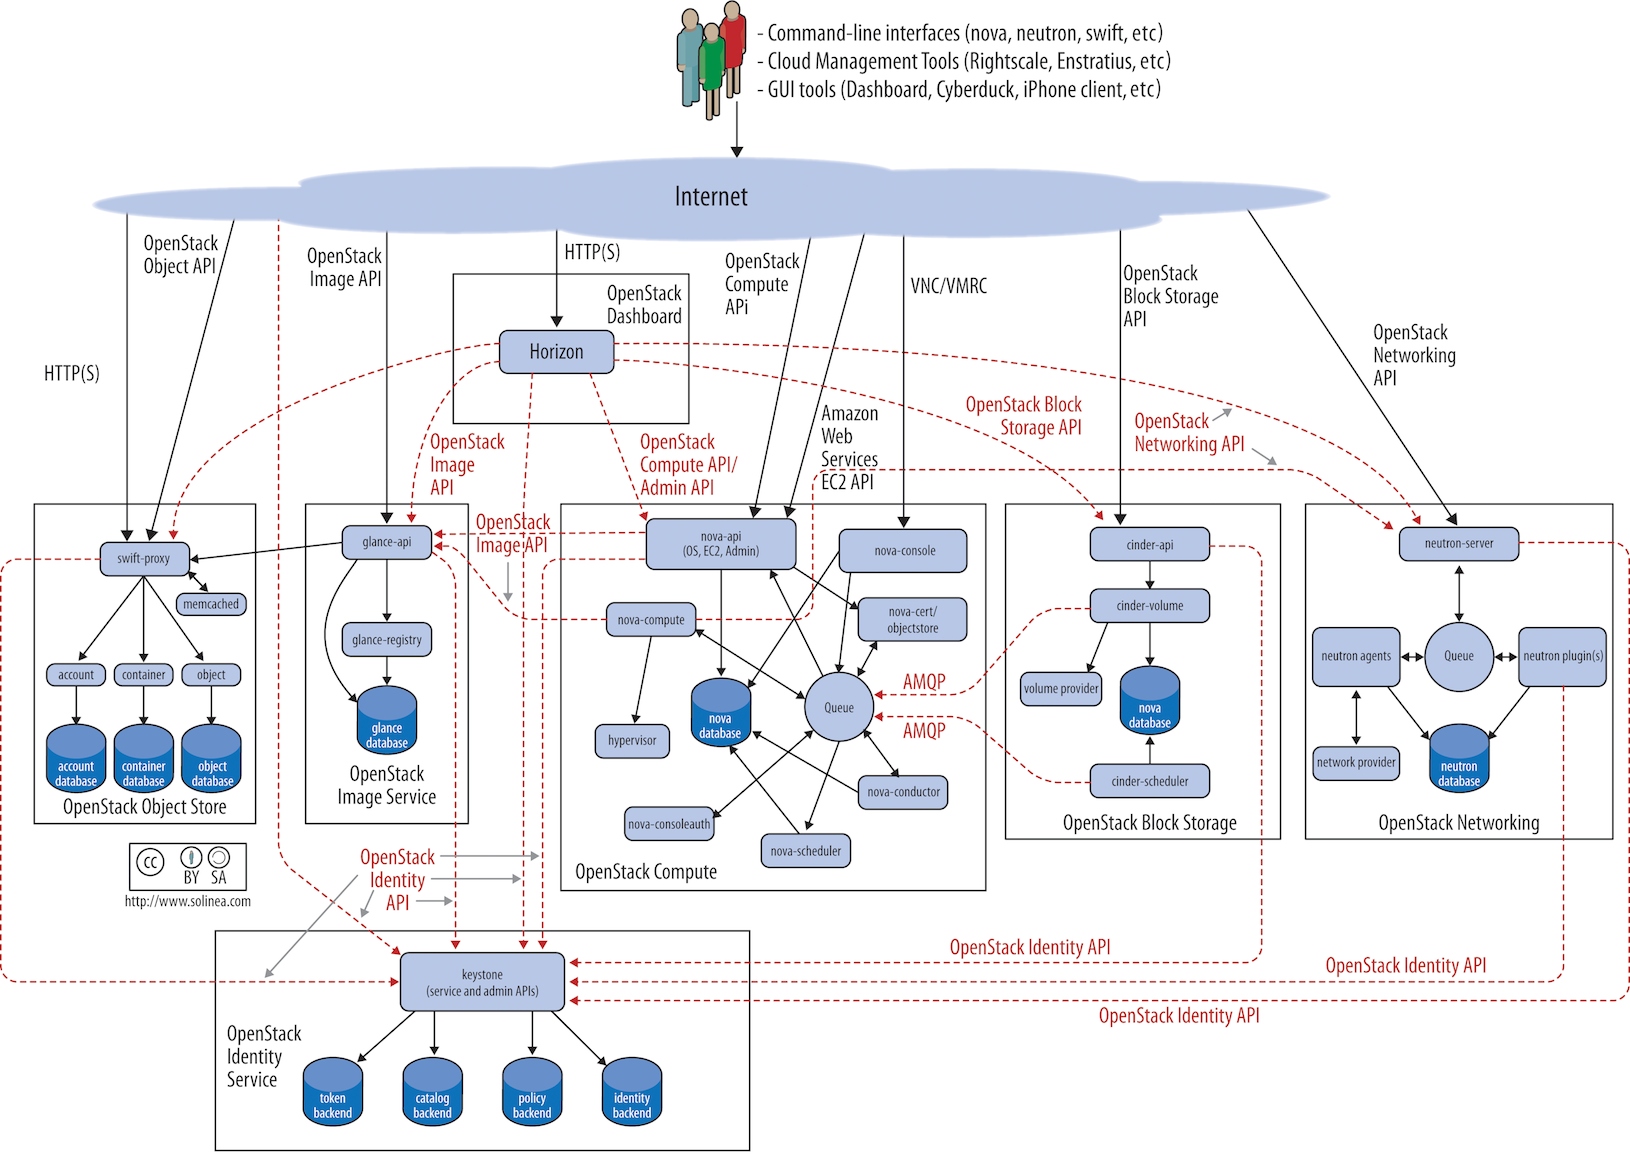
\includegraphics[width=0.9\textwidth]{openstack_logical}
    \label{fig:figure12}
    \caption{Logical Architecture of the OpenStack Components}
\end{figure}


\newpage
\subsection{OpenStack at the Edge}

Several open source communities have been formed to realize Edge computing use-cases using OpenStack. Most architectures use a Cloud and an Edge part that need to run synchronously to achieve the objectives. The key challenges in realizing openstack at the edge is that the components of openstack require large memory footprint along with the messaging and database infrastructure that runs as backbone for openstack services. This cannot be afforded when deploying at the Edge devices which have limited resources. The idea has been to optimize the openstack services to fit the requirements of the Edge device constraints. Few examples of open source effors in this area include Akraino, EdgeX Foundry, StarlingX and a few more. The figure~\ref{fig:figure13} shows the representation of openstack services at the centralized DC and the edge devices. Depending on the computational capability of the edge device, it can be hosted as Large, Medium or Small Edge \cite{osedge}.

\begin{figure}[h!]
    \centering
    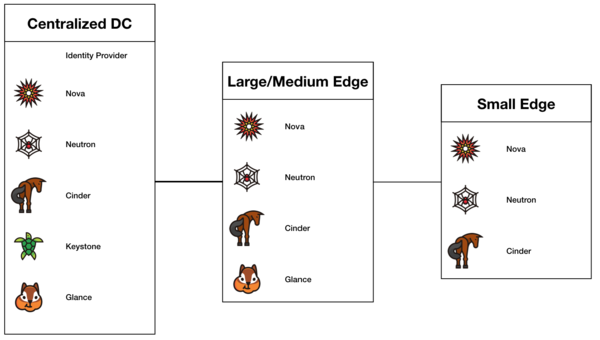
\includegraphics[width=0.9\textwidth]{openstack_edge}
    \label{fig:figure13}
    \caption{OpenStack Components for Edge Computing}
\end{figure}

The component services/daemons for each OpenStack can also be further customized based on the size of the Edge Device as illustrated in~\ref{fig:figure14} derived from \cite{osedge}.

\begin{figure}[h!]
    \centering
    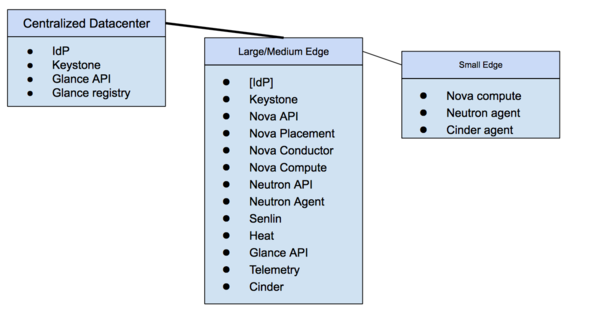
\includegraphics[width=0.9\textwidth]{openstack_edge_services}
    \label{fig:figure14}
    \caption{OpenStack Services for Edge Computing}
\end{figure}



\subsection{Kubernetes for NFV}
	
\begin{flushleft}
    Kubernetes is a production-grade, open-source infrastructure for the deployment, scaling, management, and composition of application containers across clusters of hosts \cite{k8sarch}. Kubernetes provides facilities to deploy and manage applications that utilize multiple containers. As highlighted in \cite{k8sarch}, the key design goals for kubernetes include portability, generality, legacy support, flexibility, extensibility, and automation possibility. 
\end{flushleft}

\begin{figure}
    \centering
    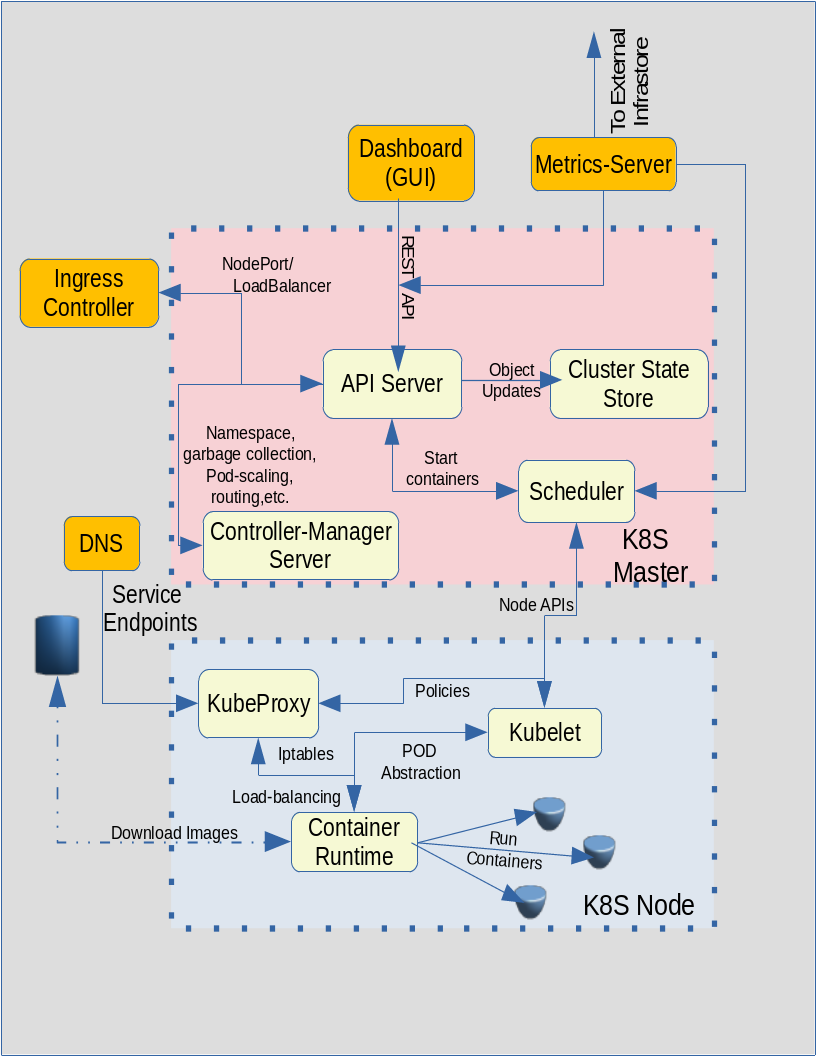
\includegraphics[width=0.5\textwidth]{kubernetes_arch}
    \label{fig:figure16}
    \caption{A block diagram representation of Kubernetes components. Derived from the description in \cite{k8sarch}}
\end{figure}

The architecture involves two types of nodes:
\begin{itemize}
    \item Kubernetes Master also known as the Cluster Control Plane
    \item Kubernetes Node that runs the containers and worloads
\end{itemize}

The Kubernetes Master provides interface to the user and maintains the state of the cluster. The control system of the master and the slave nodes work on the level-based principle wherein they act on drivin the state of the system to a desired state. They react to changes in the state through events and avoid redundant operations and minimizing reaction latency \cite{k8sarch}.
The Master node components can either be all run in a single machine or can be distributed to achieve high availability and load balancing capabilities.
The fundamental unit of kubernetes deployment is called a "POD" which is a group of containers running on the Kubernetes nodes.


The Master node comprises of the following components:

\begin{enumerate}
    \item \textit{API Server}
        It exposes the administrative functions of the Kubernetes cluster through REST API. 
    \item \textit{Cluster State Store}
        A service like etcd that stores all cluster related information persistently in a key-value format.
    \item \textit{Controller-Manager Server}
        Most of the cluster functions like creation, lifecycle management, garbage collection and the API business logic are implemented by Controller Managers. The Controller Manager is a daemon that watches the kubernetes state and makes changes to achieve the desired state. Kubernetes ships with controllers like \textit{replication controller, endpoints controller, namespace controller} and \textit}{serviceaccounts controller} \cite{k8scntmng}.
    \item \textit{Scheduler}
        The Kubernetes scheduler is responsible to choose from a set of hosts to start a set of containers for an application on request. The user can specify constraints on resource availability, Quality of Service, affinity and anti-affinity which are taken into account by the scheduler for allocation. The Scheduler also watches unscheduled PODs and binds them to nodes \cite{k8sarch}. 
\end{enumerate}

The Kubernetes node components provide the required services to run applications on containers or a group of containers(PODs). It includes the following 3 main components:

\begin{enumerate}
    \item \textit{Kubelet}
        Kubelet implements the PODs and Node APIs. PODs can host multiple containers with shared storage volumes and network infrastructure. The POD contains all the necessary resources for the application to run. All containers in a POD share a single IP address and port space and a "localhost" address is used to communicate with each other. The PODs are identified by a unique ID UUID and bind to a node until terminated. In case of faults, a new identical POD is created and the earlier POD is not rescheduled \cite{k8spod}. Through the Node APIs, Kubelet provides the essential mechanism for admission control. 
    \item \textit{Container runtime}
        Every node has a container runtime responsible for getting the images and running the containers \cite{k8sarch}. The container runtime is a logical equivalent of a hypervisor in virtualization. A CRI (Container Runtime Interface) integrates with Kubelet with the help of specifications, protobuf API and libraries that provide service management, request management and caching and error management services \cite{k8scri}. Kubernetes currently supports following CRIs:
        \begin{itemize}
            \item Docker
            \item CRI-O
            \item frakti
            \item rktlet
            \item cri-containerd
        \end{itemize}
    \item \textit{Kube Proxy}
        The kube proxy provides a mechanism to group PODs and apply iptables policies and load balancing. The services are discovered through interaction with the DNS service.
\end{enumerate}

In addition to the above components, a Kubernetes system can also use additional components to help its operations:
\begin{enumerate}
    \item \textit{DNS} - Provides name service for service PODs
    \item \textit{Ingress Controller} - Proivdes access to services by external entities
    \item \textit{Metrics-Sever} - Provides collection and monitoring of metric data on running PODs
    \item \textit{Dashboard} - Provides a Graphical User Interface for the administrative tasks on the Kubernetes cluster.
\end{enumerate}

Kubernetes is a relatively new introduction to the NFV world. The network functions that are made to run in a container are referred to as Containerized Network Functions (CNFs). The CNCF (Cloud Native Computing Federation) is constantly striving to enable Kubernetes as an alternative technology to realize NFV Infrastructure. [\cite{sharma16}] provides a comprehensive comparison of Containers vs Virtual Machines and establishes that containers are a viable option for realizing NFV use-cases.

\subsection{Kubernetes at the Edge}

\begin{flushleft}
The below diagram shows the architecture of Kubeedge project, an initiative to develop Edge platform using Kubernetes. The details about the project and its source can be found in \cite{kedge}.
\end{flushleft}

\begin{figure}[h!]
    \centering
    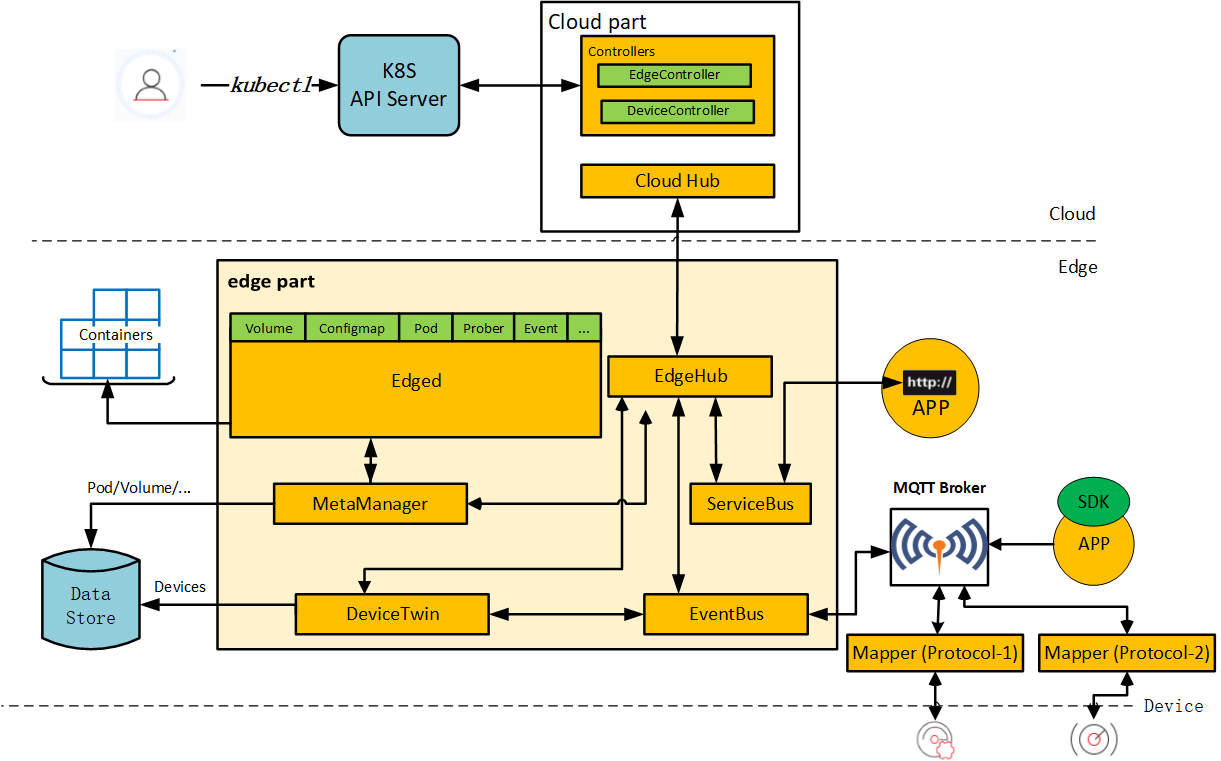
\includegraphics[width=0.9\textwidth]{k8s_edge}
    \label{fig:figure14}
	\caption{Architecture of the KubeEdge project. From \cite[What is KubeEdge]{kedgedoc}}
\end{figure}

\begin{flushleft}
The architecture as shown in Figure 14 consists of two parts:
\end{flushleft}
\begin{enumerate}
    \item \textbf{The Cloud Part}
	    The components that run in the data center and provides mechanisms for the edge part to synchronize with the cloud part. The cloud part consists of the following components:
        \begin{itemize}
            \item \textit{Edge Controller} - interfaces with the Kubernetes API Server and syncs with the events and updates with the edge core.
            \item \textit{Device Controller} - Updates and syncs device status using device model and device instance. 
            \item \textit{Cloud Hub} - Prepares the platform for communication between the cloud and the edge (websocket, channelQ, messages)
		\end{itemize}
    \item \textbf{The Edge Part}
        The components that run on the edge device and interact with the end-user equipment. It synchronizes with the cloud part for functions like device management and service updates. It comprises the following components:
		\begin{itemize}
            \item \textit{EdgeD} - A daemon that manages the life cycle of the pod/s on the edge node. It proposes to include a CRI as a replacement for the current docker runtime to ensure a lightweight runtime and also provide options to choose from multiple container runtimes.
            \item \textit{EventBus} - Is responsible for sending/receiving messages over MQTT to/from external clients.
            \item \textit{MetaManager} - Responsible to process, store and query messages between the Edgehub and the EdgeD. 
            \item \textit{Edgehub} - Interacts with the Cloud Hub on the cloud part either through web-socket or using QUIC protocol. The functions include reporting device and edged status to the cloud and sync with cloud-side resources.
            \item \textit{DeviceTwin} - Supports Device management through storing and querying device status, health check, message distribution and membership management.
	    \end{itemize}
\end{enumerate}

\section{Conclusion}

Cloud computing, Virtualization and Containerization have enabled commoditization of communication services. The ability to move workloads to virtual machines and containers has helped flexibility and scalability necessary for new types of services. Some of these services would now be able to utilize the computational power and data availability at the edge of the network. There has been humongous efforts in the standards bodies and open source communities in moving the Edge computing technology forward. While OpenStack leverages virtualization technologies, Kubernetes uses containerization to realize the functional blocks of the Edge computing system. The open source solutions try to address the hard requirements through auxiliary projects and optimizations. The middleware layers provide facilities to utilize the underlying optimization in an automated fashion to realize the infrastructure as needed by the application. An important goal of the architectures presented is to make application development as simple as possible by not exposing the complexities of the underlying infrastructure through separation of concerns. The Management plane and Control plane work in tandem with the Application to produce the desired results on the Data Plane.



%
%===============================================================================
% LATEX-Dokument: Literaturverzeichnis
%===============================================================================
%
\newpage
\phantomsection
% Einstellungen f\"{u}r Literaturverzeichnis
\addcontentsline{toc}{section}{\bibname}

\bibliographystyle{IEEEtran}
% argument is your BibTeX string definitions and bibliography database(s)
\bibliography{\meta/Literature/reference}
% Nutzung von Bibtex:
% hier den bib-file einbinden
%
% GATHER{bibfile.bib}
% \footnotesize
% \bibliography{bibfile}
% ansonsten: bbl als tex Datei einbinden
 %\input{KTR-Seminar-Literatur.tex}
%===============================================================================
% LATEX-Dokument: Literaturverzeichnis
%===============================================================================
%
\end{document}
